\documentclass{article}
\usepackage{lmodern}
\usepackage[T1]{fontenc}
\usepackage[english,activeacute]{babel}
\usepackage{mathtools}
\usepackage{biblatex}
\usepackage{csquotes}
\usepackage{graphicx}
\usepackage[]{algorithm2e}

\setcounter{tocdepth}{5}
%\setcounter{secnumdepth}{5}

\title{User Behavior Analysis in Campus Area Networks through Kohonen Self Organizing Feature Maps}

\author{Nelson Victor Cruz Hern\'andez }

\date{June 2017}

\begin{document}

\maketitle






\section{Introduction} % level 1
Inbounds

\subsection{Background} % level 2

\subsection{Justification} % level 2

\subsection{Problem} % level 2

\subsection{Hypothesis} % level 2

\subsection{Objectives} % level 2

\subsubsection{General Objectives} % level 3

\subsubsection{Particular Objectives} % level 3







\section{State of the Art} % level 1

\subsection{Machine Learning Algorithms and Computer Security} % level 2

\subsection{Profiling  and User classification} % level 2






\section{Theorical framework} % level 1

\subsection{Proxy} % level 2

\subsection{Machine Learning algorithms}	 % level 2

\subsubsection{Learning methods} % level 3

\paragraph{Supervised Training Methods} % level 4
Obtain the information from "Artificial Neural Networks An introduction Kevin L. Priddy and Paul E. Keller" Chapter 2.1

\paragraph{Unsupervised Training Methods} % level 4
Obtain the information from "Artificial Neural Networks An introduction Kevin L. Priddy and Paul E. Keller" Chapter 2.3
                                                                                                                                                                                                                                                                                                                                                                                                                                                                                                                                                                                                                                                                                                                                                                                                                                                                                                                                                                                                                                                                                                                                                                                                                                                                                                                                                                                                                                                                                                                                                                                                                                                                                                                                                                                                                                                                                                                                                                                                                                                                                                                                                                                                                                                                                                                                                          \subsubsection{Gaussian function} % level 3

\subsection{Self-organizing Maps} % level 2
The Self-Organizing Map algorithm performs a nonlinear, ordered, smooth mapping of high-dimensional input data manifolds onto the elements of a regular, low-dimensional array [25]. The algorithm converts non-linear statistical relationships between data elements in a high-dimensional space into geometrical relationships between elements in a two-dimensional map (lattice), called the Self-Organizing Map (SOM)[1]. A SOM can then be used to visualize the clusters, of an input space. Each element at SOM is a neuron, and is a representation of a multidimensional vector with a cartographic position denoted with x and y. If elements in the input space are characterized using k parameters and represented by k-dimensional vectors, each neuron in the SOM lattice is also specified as k-dimensional vector.

\subsubsection{Learning} % level 3
In the learning or training phase, the neurons in SOM algorithm try to model the input space. 
SOM algorithm differ from other artificial neuronal networks as they apply competitive learning and use a cooperative schema. 

--- OPTION 1 ---
Opposed to error-correction learning, in which each element $s_n$ in the training dataset $S$ is evaluated by the neuronal network connections $W(w_1, w_2,...,w_n)$ and the result $r$ is compared against a predefined threshold to decide if the result matches the expected output and an adjustment to $W$ is needed, in competitive learning each element $e_n$ of the training data set $E$ is shown to every neuron $N(n_1,n_2,...,n_n)$ in the SOM lattice Each neuron $n_n$ calculates a response $h$ to the shown element, based on a preselected distance measure. The neuron that gives the best response is called the winning neuron or best matching unit (BMU).
--- FINISHES OPTION 1 ---

--- OPTION 2 ---
Opposed to error-correction learning, in which the evaluation result of an element in the training dataset may result in the complete adjustment of the neuronal network connections, in competitive learning each element $e_n$ int the training data set $E$ is shown to every neuron $N(n_1,n_2,...,n_n)$ in the SOM lattice, the response is calculated through a preselected distance measure, the neuron that gives the best response is called the winning neuron or best matching unit (BMU) and gets it's vector values updated.
--- FINISHES OPTION 2 ---

Suitable distance measure should be stablished in order to find the BMU. Two common used distance measures are dot-product measure and euclidean distance.
For using dot-product measure, lattice neurons $N$ and training elements $E$ should be normalized. Normalization of a vector $V(v_1, v_2, v_3,...,v_n)$ is a process of transforming it's components into
$(\frac{v_1}{\sqrt{v_1^2+v_2^2+...+v_n^2}},
\frac{v_2}{\sqrt{v_1^2+v_2^2+...+v_n^2}},
...,
\frac{v_n}{\sqrt{v_1^2+v_2^2+...+v_n^2}}
)$
 so that the modules of the normalized vector is unity. The dot-product of the input vector is calculated against all the neurons in the lattice, where dot-product of two vectors $Y(x_1, x_2, x_3,..., x_n)$ and $Z(z_1, z_2, z_3,..., z_n)$ is defined by: 
 
 
\begin{equation}
X \cdot Z = (x_1 \cdot z_1 + x_2 \cdot z_2 + x_3 \cdot z_3 + ... + x_n \cdot z_n)
\end{equation}
 
 
 Using this measure means that BMU is the one that gives the maximum dot-product value.
 
 In the other hand, euclidean distance measure does not need vector normalization and the BMU is defined for the minimum obtained distance. For two vectors $Y(y_1,y_2,...,y_n)$ and $Z(z_1,z_2,...,z_n)$ euclidean distance is given by:
 
\begin{equation}
D = \sqrt{(z_1-y_1)^2 + (z_2-y_2)^2 + ... + (z_n-y_n)^2}
\end{equation}

 Once a BMU is obtained, it's $k$-dimensional values are adjusted so in the future it responds better to a similar input $e_n$.

As SOM algorithm is not just a classification algorithm but also a clustering algorithm, a way of maintaining the dimensional relationships between elements in the same geometrical area is to get their $k$-dimensional values updated at the same time as the BMU does. This update is known as a cooperative schema, and it only works on neurons that are in the vicinity of the BMU defined by a neighborhood function.

\paragraph{Neighborhood Function} % level 4

\paragraph{Learning Function} % level 4

\subsection{Redes de Computadoras} % level 2

\subsubsection{Local Area Network (LAN)} % level 3

\subsubsection{Campus Area Network(CAN)} % level 3

\subsubsection{Network topology} % level 3

\subsubsection{OSI Model / TCPIP} % level 3

\subsubsection{Network Security} % level 3

\subsubsection{Intrusion Detection Systems} % level 3






\section{Methodological Development} % level 1


\subsection{Experiment context} % level 2
Experiment was carried out on a Campus Area Network (CAN) that has a 16-bit network and a Windows domain controller, using a HTTP proxy. Among campus applications web and remote apps are included.
Email service is provided by Microsoft Exchange Server which is hosted outside the campus network.
The target users were full-time professors who had a computer with a static IP address and a wireless access with a dynamic IP address.
Five full-time professors (hereafter denoted as users) were selected for the experiment. For each one, real usage traffic was captured for inside and outside campus activities during a two labor weeks, and then processed.






\subsection{Explanation} % level 2
In this work Self Organizing Maps algorithm is used to create an user pattern inside a Campus Area Network. Experiments are divided in three phases: network data capture, data processing and pattern evaluation.

For network data capture phase, a set of raw packages is obtained for each user through tcpdump library, process is explained in [Parres, XX].

For data processing phase, each set of raw packages is arbitrary divided in build, train and evaluate sets.
Each set is processed to compress raw packages into chunks of a five minutes window $t$ represented by three metrics that involve communication protocol, origin and destination ip and total transmitted bytes.
From the obtained build data set, a fixed number of elements $n$ is randomly selected, this number defines the size of the Self Organizing Map lattice $(n x n)$.
For lattice training, a fixed number of elements $e$ is randomly selected from train data set. Self Organizing Map is considered to be fully trained, after a cycle of ten epochs, as a result of this phase an user network behavior pattern is obtained.

Evaluation phase is done by joining different user network behavior patterns in one lattice, similar to a blanket filled of patches in which each patch is represented by an user network behavior pattern, creating what we define as the organization pattern. An organization evaluation set is build by all the user evaluation sets that belong to each user that conforms the organizational pattern. Each element of the organization evaluation set is shown to the organization pattern, resulting best matching unit is compared against the original user of the shown element to the lattice. Correct match of the user attribute of the shown element and user attribute of the best matching verifies that the shown element is able to recognize it's original user among others. The complete process of an experiments is shown in Fig. 1.

	\begin{center}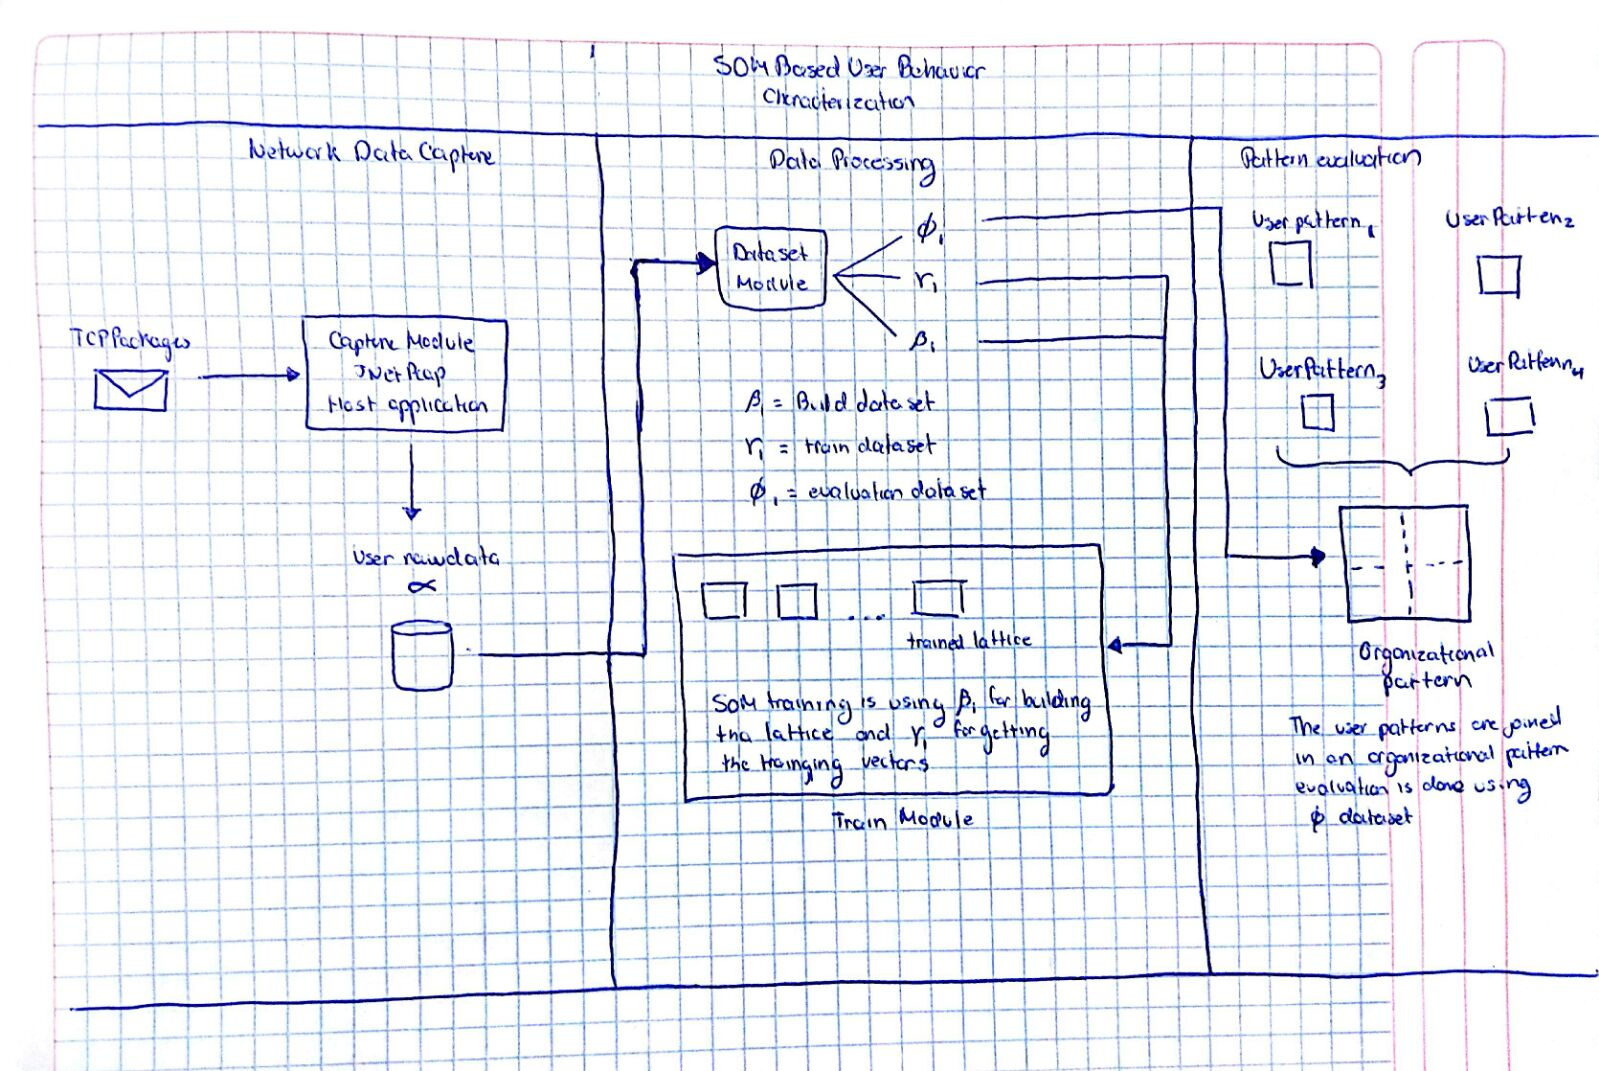
\includegraphics[scale=0.2]{fig-two} \end{center}

For each phase in the process one or more modules were build, each module's output is used as an input for the next phase corresponding module.


\subsubsection{Network data capture} % level 3
Network data capture phase duration was at least of two labor weeks,  in which network traffic was captured from each user's computer.
Capture module was build using jNetPcap, which works as a client application that once installed enables to capture continuously user network data in an IP packet format and save it in files of twenty megabytes each, naming them with file's creation timestamp. Average size of complete raw captured traffic for each user is three gigabytes, involving more than four million packages. Each register contains the characterization of a network connection by eight parameters: origin IP, destination IP, used protocol, local used port, remote used port, total transmitted bytes in the package, timestamp and the connection-way which establishes if the package is coming from local to remote (out), or from remote to local (in).



\subsubsection{Data processing} % level 3
Data processing phase is divided in four stages: a) Raw data partition, b) Data sets creation, c) Self Organizing Map algorithm implementation and d) User network behavior pattern creation. Two modules were build for this phase, data set and train module. Data set module involves Raw data partition and Data set creation stages and Train module involves Self Organizing Map algorithm implementation and User network behavior pattern creation.




\paragraph{Raw data partition} % level 4
As explained in section 3.3 Self Organizing Map algorithm is a not supervised algorithm due different information is needed en each phase of the algorithm. Complete user raw captured data $\alpha$ is divided in three subsets: build package set $\beta$, train package set $\gamma$, and evaluation package set $\phi$. As data captured is divided in files containing continuous user network data, dividing the complete raw data set in subsets, enables having en each subset different days of user behavior. Complete raw data set is divided equally between each subset.

\begin{equation}
\alpha = \beta \cup \gamma \cup \phi
\end{equation}




\paragraph{Data set creation} % level 4
Using TCP package as the working unit is not possible due the great volume of packages, and time consuming for processing each one individually [Reference, XX].

Instead, package sets $[\beta,\gamma,\phi]$ are individually processed and turned into chunks. The obtained chunks are the the working units and conform the different data sets, Build data set $\beta_1$, the Train data set $\gamma_1$ and the Evaluation data set $\phi_1$ respectively. Fig 2 shows the process of dataset creation.

	\begin{center}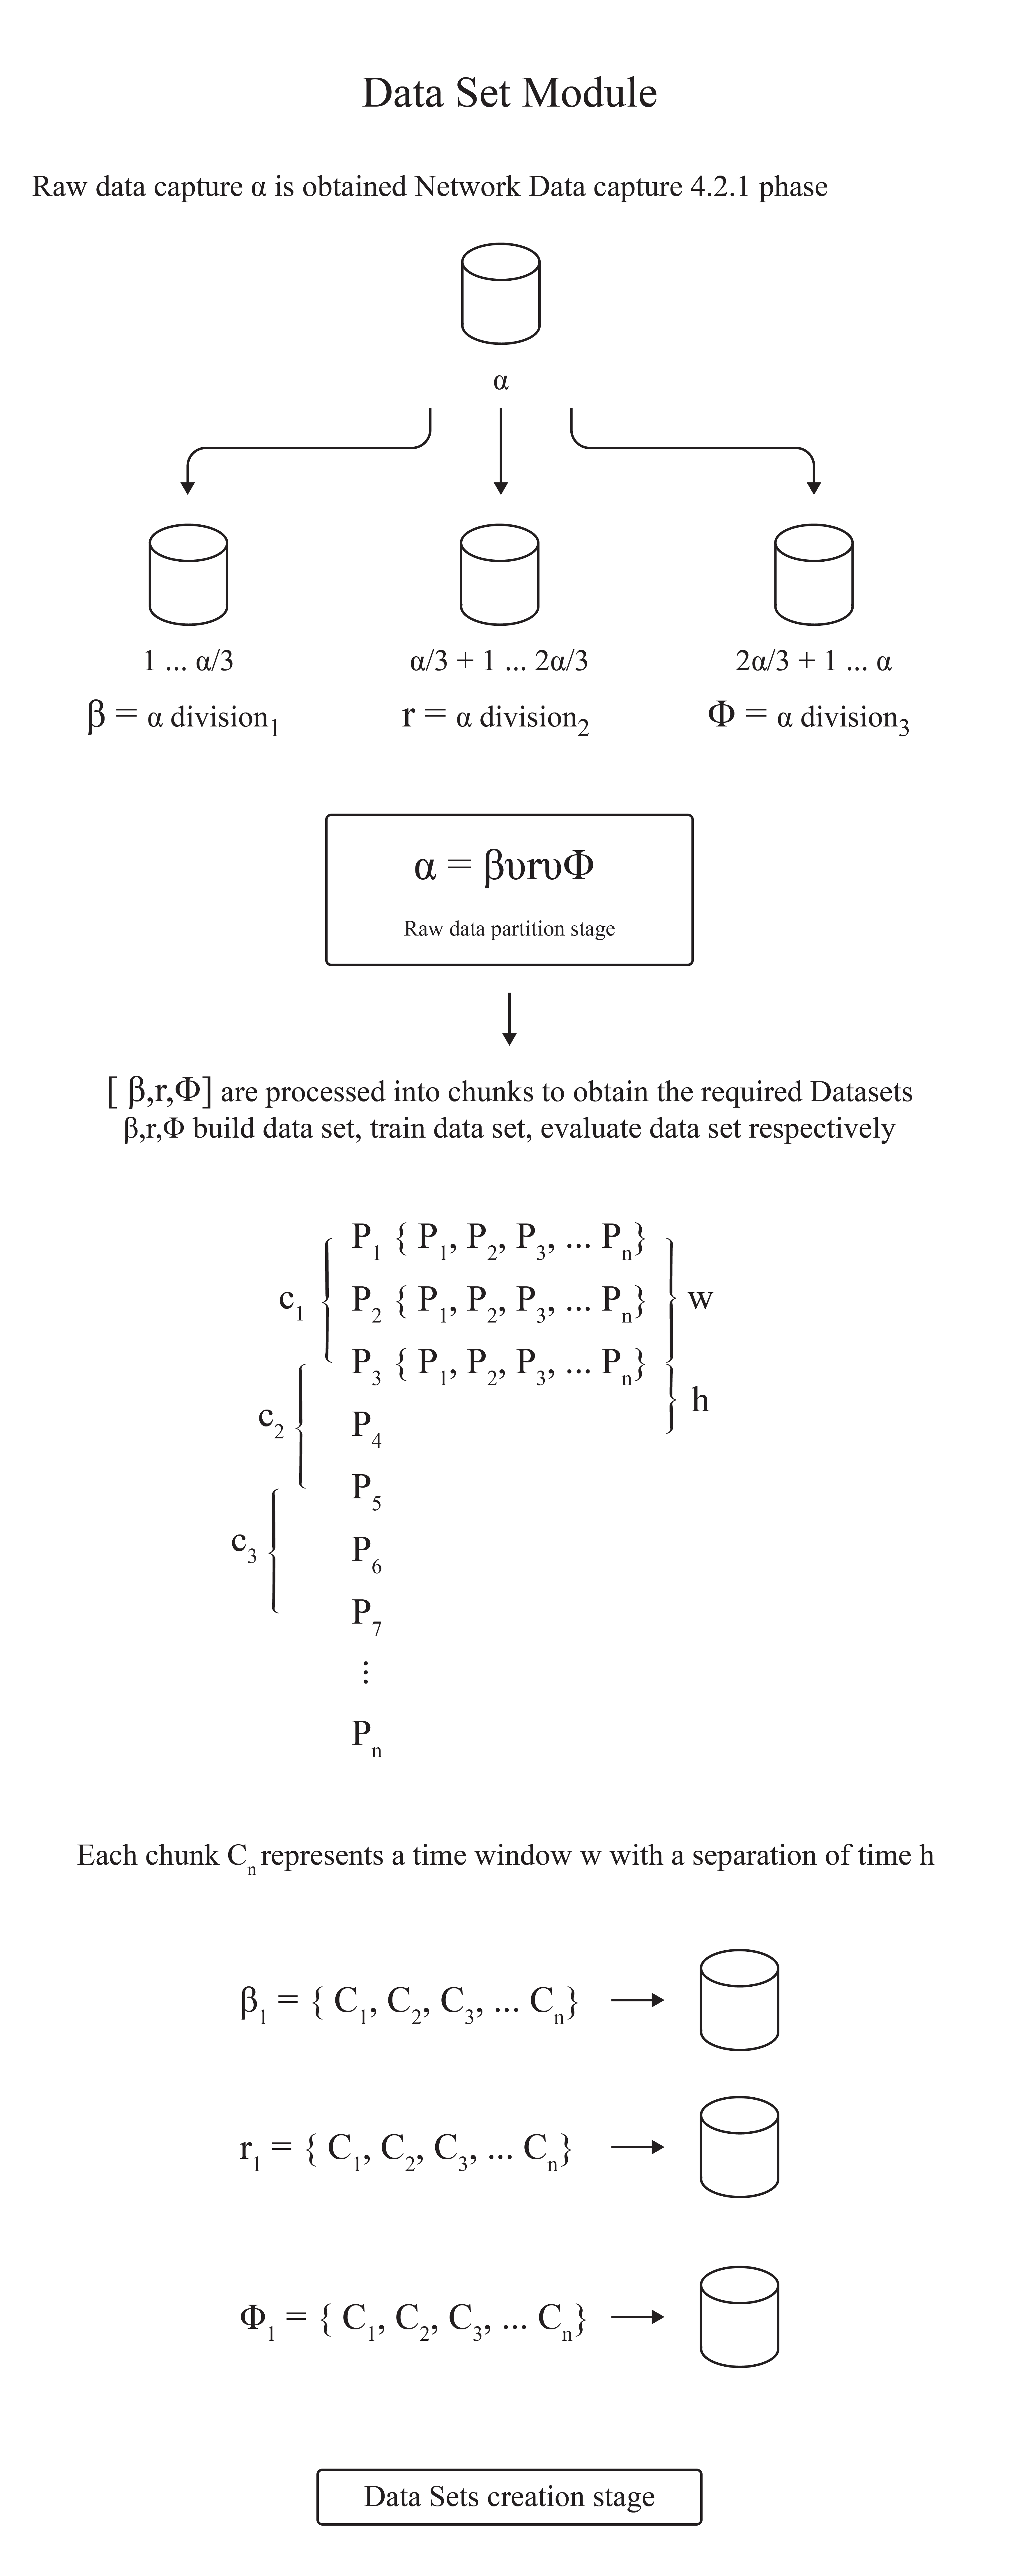
\includegraphics[scale=0.2]{fig-three} \end{center}
	
Each chunk $C$ is defined with the following characteristics: a) It is conformed by one or more packages $C_n(p_1, p_2,...,p_n)$ that have a continuity in their timestamp field, b) It has a fixed time window $w$ but does not have a fixed number of packages, c) The difference between $p_n$ timestamp and $p_1$ timestamp is less or equal to the fixed time window $w$ and d) The difference between start timestamps of consecutive chunks is a fixed time $h$.

The elements in a package set are processed one by one, as follows:

\begin{enumerate}
  \item Total packages in the package set is obtained and assigned to $n$, the index of the element that is being processed is assigned to $i$ and a global index that holds the package index in which the chunk $C_n$ start is assigned to $g$.
  \item First chunk $C_1$ start timestamp $t_1$ is set with the timestamp of $p_1$ and finish timestamp $t_2$ is calculated ($t_1 + w$).
  \item While $i$ < $n$ and $p_n$ timestamp is less than $t_2$, $p_n$ is added to the package chunk's collection and $i$ is assigned to the next element in the set, otherwise the $p_n$ is not added to the package chunk's collection, and the chunk is complete.
  \item $C_1$ is added to the chunks data set's collection.
  \item New start timestamp is calculated $t_1 + h$ and assigned to the new chunk $C_n$.
\end{enumerate}
Steps 2 to 5 are repeated while $g$ < $n$.

Processing packages as a chunk allows getting a summary of the information sent in a $w$ period of time, such as: total bytes sent, total bytes sent through TCP and UDP protocol, total bytes sent for web traffic destination along 80, 443 and 3128 ports and as we are working inside and Campus Area Network total bytes sent to internal destination (same backbone ip, our case 148.201.X.X). This data is condensed into three metrics: a) TCP-UDP metric, represents the ratio between total bytes sent through both protocols and total bytes sent in the chunk , b) Internal IP metric, represents the ratio between total bytes sent to CAN proxy ip and total bytes sent in the chunk and c) Web traffic metric, represents the ratio between data sent through web ports, and and total bytes sent in the chunk.
Obtained metrics are the $k$-values of the neurons in the Self Organizing Map lattice.




\paragraph{Self Organizing Map algorithm implementation} % level 4
Self Organizing Map basic algorithm is defined as follows.
\begin{enumerate}
\item Initialization. Choose random elements for the initial weight vectors $w_j$.
\item Sampling. Select a sample training input vector $x_n$ from the input space.
\item Matching. Find the winning neuron $L(x)$, that has it's weight vector closest to the input vector $x$.
\item Updating. Apply the weight update equation $\Delta w_j=\eta(t) \times \kappa(t) \times (x_i - w_j)$; where $\eta(t)$ is a gaussian neighborhood function and $\kappa(t)$ is the learning rate.
\item Continuation. Keep returning to step 2 until the feature map stops changing.
\end{enumerate}

Each element in the SOM lattice has a weights vector $V(v_1, v_2,..., v_n)$ of three elements, $v_1$�represents the TCP/UDP metric, $v_2$ represents the Internal IP metric and $v_3$ represents the Web traffic metric.

To define the the size $n$ of the lattice, experiments were done with 50, 75, 100 and 125 elements. Table 1. shows the time needed to train the lattices. As it can be seen as more elements in the lattice, time increases, but the results when comparing the obtained patterns against other users are very similar.The lattices used for the experiments were build using XX elements,  obtained randomly from the Build data set $\beta_1$ and ordered in a square distribution.

For the evaluation phase, a new set based on the Training data set $\gamma_1$ was obtained. The average number of elements on the train data set of each user was 56,496 elements, the created data set, was conformed by 100,000 elements, guaranteeing that each element was evaluated at least one time.

Best matching unit evaluation was obtained using Euclidean distance. The gaussian neighborhood function was used with an initial neighborhood radius of ($\frac{n}{2}$), decreasing linearly to 1 at the end of the training. The learning rate was chosen to be 1 and reduced to 0 at the end of the training.




\paragraph{User network behavior pattern creation} % level 4
The train module implements the SOM-based approach for user characterization. In the training phase 10 epochs are used to process the lattice. After this phase, an user network behavior pattern is obtained. This pattern may differ between patterns obtained from the same user, because of the random selection of the build elements. Fig 3 shows lattice training during it's initial phases until it get's completely trained.

\begin{center}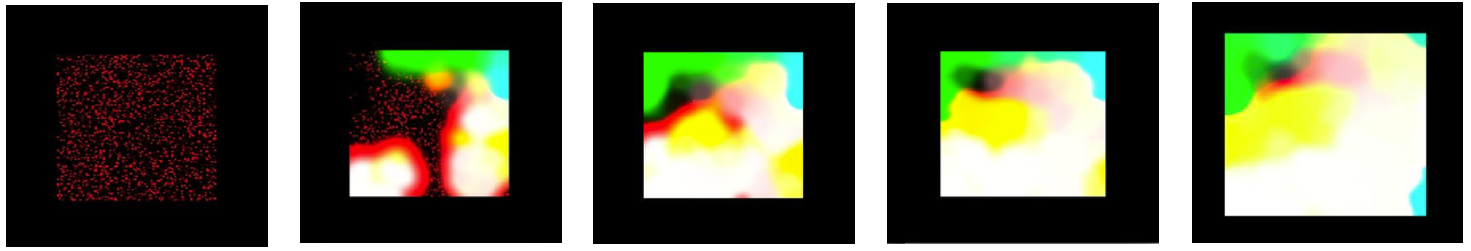
\includegraphics[scale=0.2]{fig-training} \end{center}





\subsubsection{Pattern evaluation} % level 3
When SOM lattice is completely trained, the elements with the same characteristics in their weights vector are grouped in the same area, denoting clusters of elements and a inherent classification. This obtained distribution of the elements along the SOM lattice, allows to classify easily new vectors, even if them were not in the the build or the train dataset [Reference, XX].

The pattern evaluation module use the capacity of the SOM lattice, of matching new input vectors to their similar ones, not for classifying a new element, but for deciding if an user behavior can be identified among others. To perform this evaluation, new elements are needed: a) an organizational pattern and b) an organization evaluation dataset. An organizational pattern is defined as a matrix of user patterns $P$, which represent an user with it's own behavior in an environment where different users with common or completely different behaviors are present. The organization evaluation pattern is a collection of evaluation data sets $\phi_1$ of the users that conform the organizational pattern, acting as a labeled evaluation data set.

Evaluation is done by showing each element of the organization evaluation data set to the organizational pattern, resulting best matching units are processed by obtaining the user pattern they belong to and compare it against the expected result. Fig 4. shows an organizational pattern of 4 users, and Fig 5. shows an organizational pattern after the evaluation.

	\begin{center}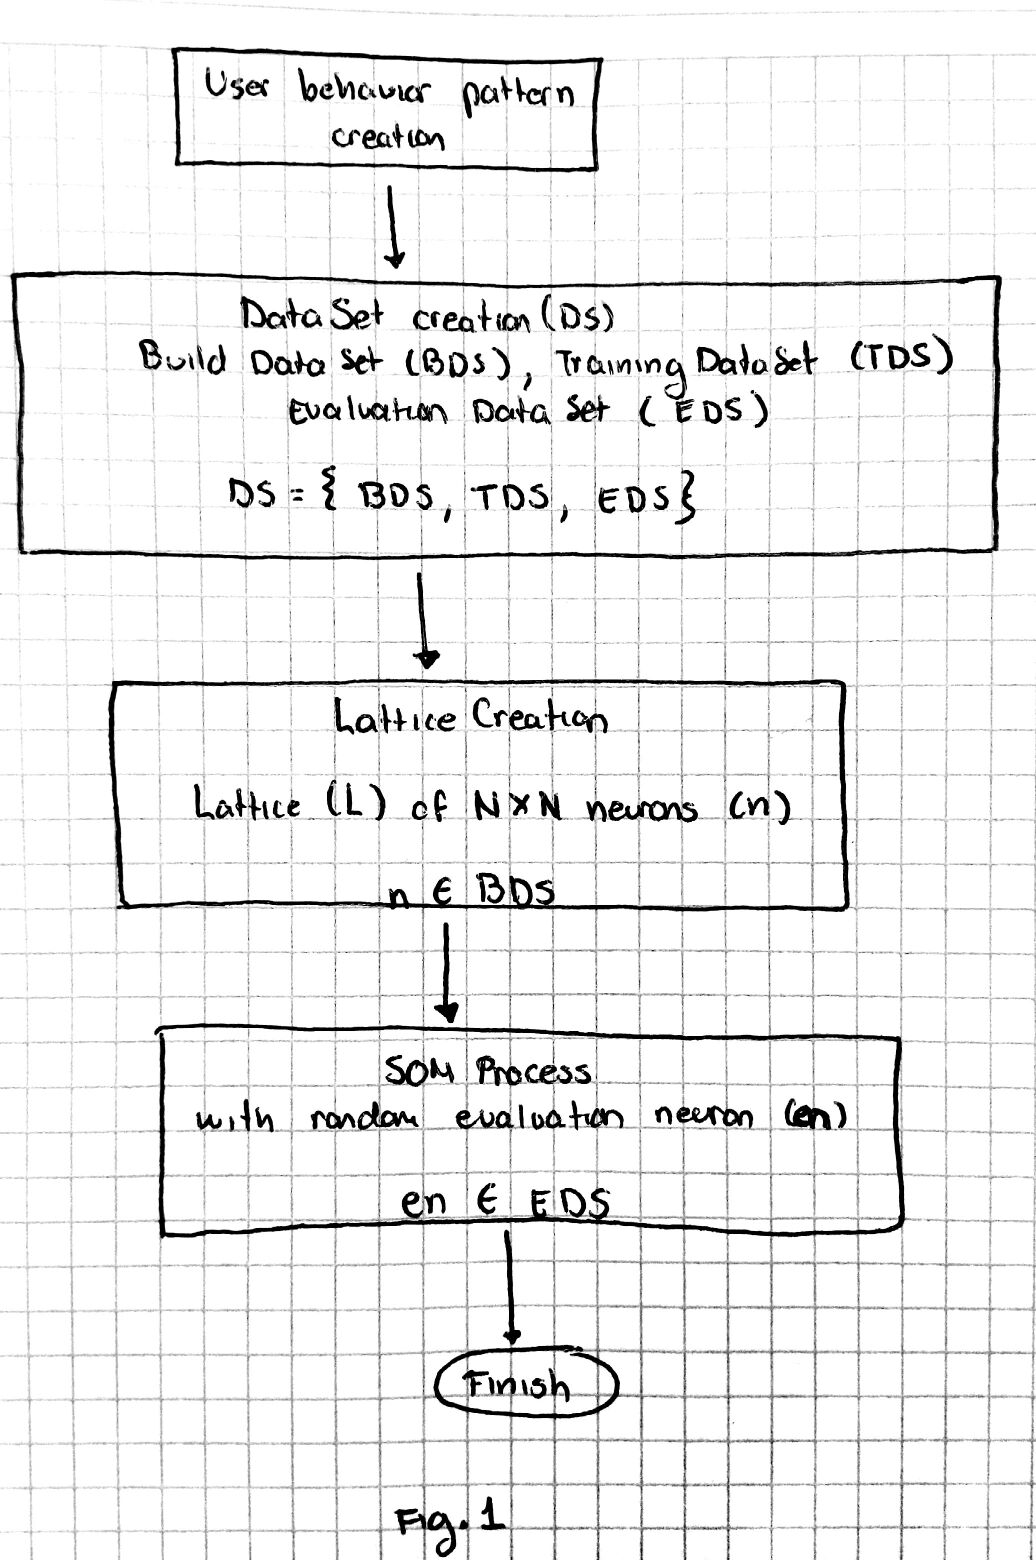
\includegraphics[scale=0.5]{fig-one} \end{center}
	
	\begin{center}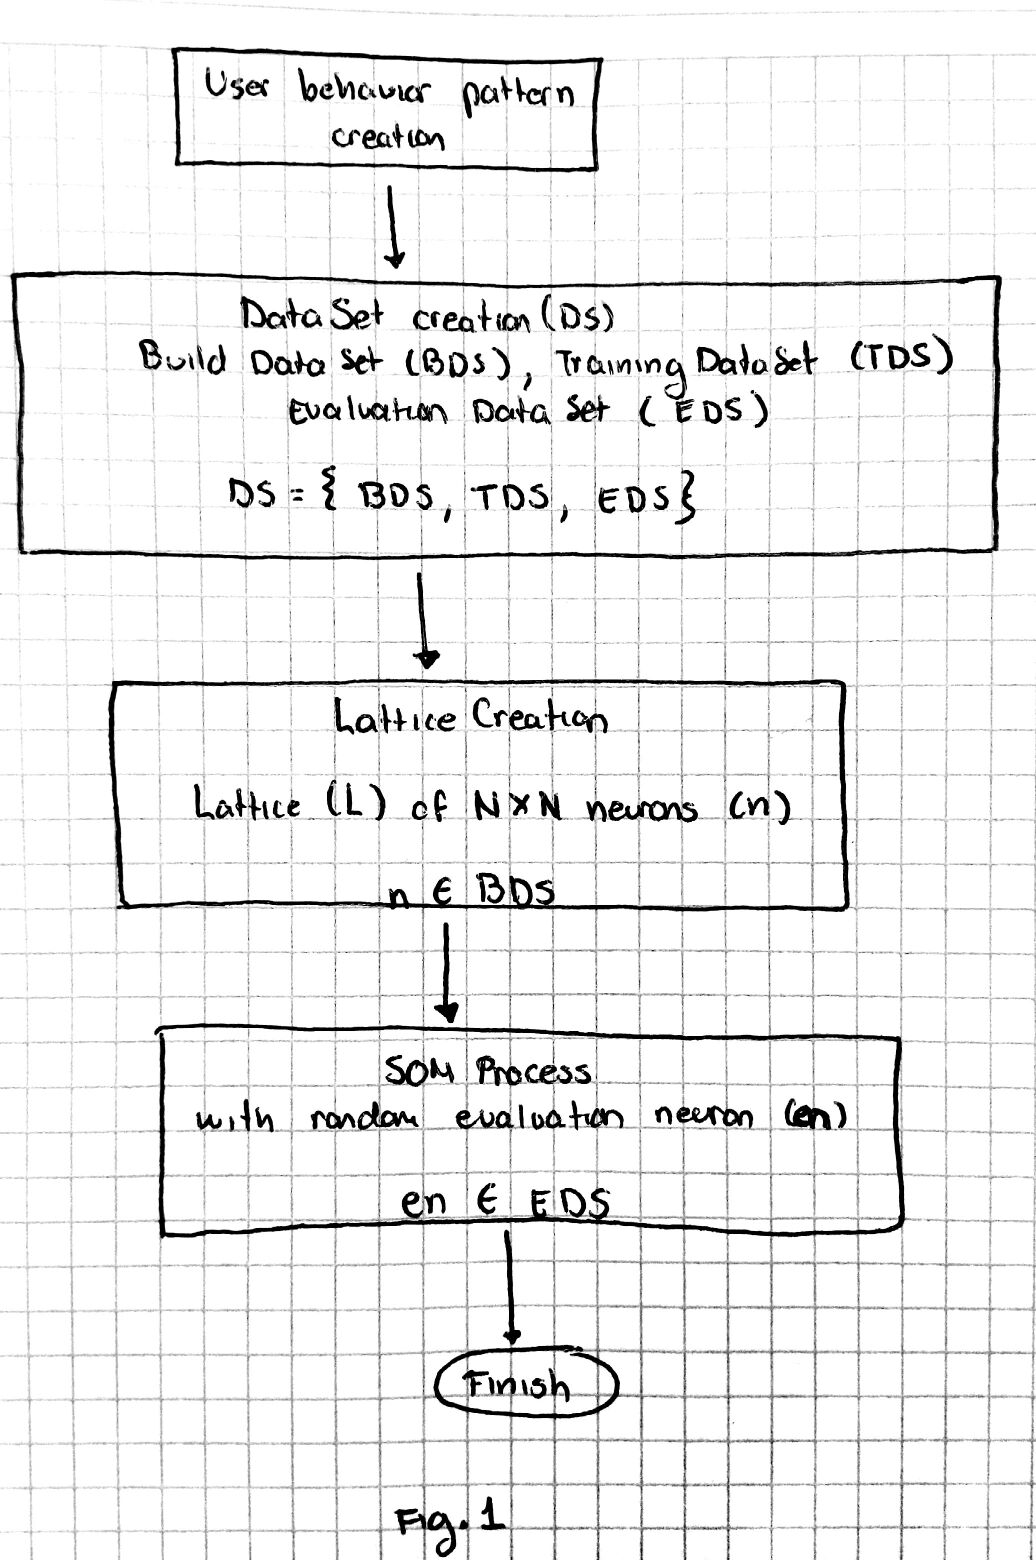
\includegraphics[scale=0.5]{fig-one} \end{center}



\section{Results and Discussion} % level 1
Results presentation, how the results are interpreted, and what we can do with data.
The results will explain, how the user is able to recognize itself in the organization map.






\section{Conclusions} % level 1

\subsection{Future work} % level 2
Due hardware limitation, SOM training is done with ten epochs. A much longer training of about one thousand epochs would give a more precise user pattern, helping in a better user detection in the organization map.
Also formulas are not completely following the standard of a gaussian function so a new implementation would be great.






\section{Bibliography} % level 1
[1] Ramadas, M., Ostermann, S.,  Tjaden, B. Detecting Anomalous Network Traffic with Self-organizing Maps.
[8] Dozono, H., Itou, S., and Nakakuni, M. (2007). Comparison of the adaptive authentication systems for behavior biometrics using the variations of self organizing maps. International Journal of Computers and Communications, 1(4), 108-116.
[25] T.Kohonen. Self Organizing Maps. Springer, third edition, 2001.



\end{document}